\documentclass[12pt]{article}
 \usepackage[margin=1in]{geometry} 
\usepackage{amsmath,amsthm,amssymb,amsfonts}
\usepackage{graphicx}
 
\newcommand{\N}{\mathbb{N}}
\newcommand{\Z}{\mathbb{Z}}
 
\newenvironment{problem}[2][Problem]{\begin{trivlist}
\item[\hskip \labelsep {\bfseries #1}\hskip \labelsep {\bfseries #2.}]}{\end{trivlist}}
 
\begin{document}
 
%\renewcommand{\qedsymbol}{\filledbox}
%Good resources for looking up how to do stuff:
%Binary operators: http://www.access2science.com/latex/Binary.html
%General help: http://en.wikibooks.org/wiki/LaTeX/Mathematics
 
\title{Homework 9}
\author{Tanner Kvarfordt - A02052217}
\maketitle
 
In the "real world" a flock is called a \textbf{tournament}. The name is intended to reflect the notion of a \textit{round-robin tournament}, as in tennis, where every player plays every other player with the convention that no ties are allowed. An equivalent notion is that of \textbf{paired comparison} of $n$ objects, where $n \in\mathbb{N}$. That is, a data set with the outcome of the comparison of every possible pair of objects recorded and the outcome is the relation \textit{is better-than} or \textit{is preferred-to} or something like that.
 
\begin{problem}{1}
Please prove that in every tournament, if a vertex is beaten it is beaten by a queen.
\end{problem}
 
\begin{proof}
Consider an arbitrary vertex $k$ in an arbitrary tournament, where $k$ is beaten by at least one other vertex. Consider, as roughly illustrated in the image below, the set of vertices, $A$, that beat $k$, where $|A|\geq1$, and the set of vertices, $B$, that $k$ beats where $|B|\geq0$. Define $W$ as the set containing all vertices of the tournament, that is, $A \subseteq W$, $B \subseteq W$, $k \in W$. \\
\begin{center}
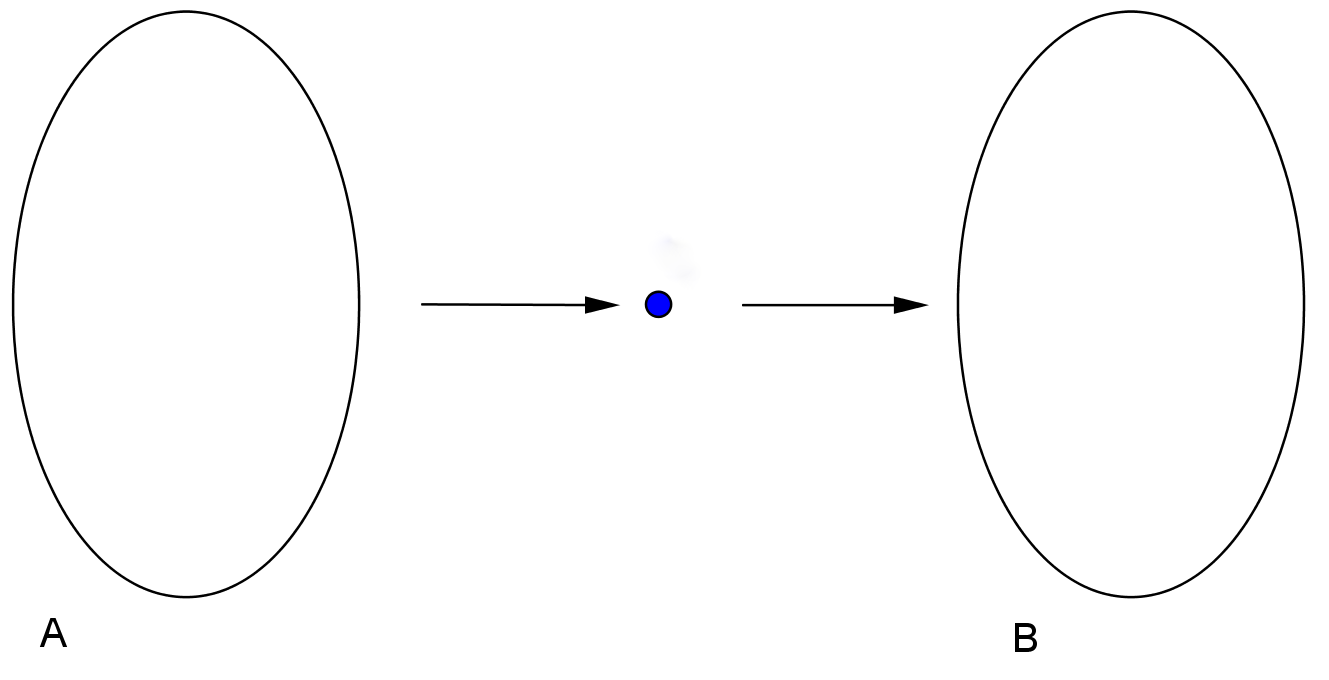
\includegraphics[scale=0.8]{Prob_1.png}
\end{center}
Consider the case where $|A|=1$. It is clear in that situation that the sole member of $A$ is a queen in the entire tournament, $W$. Now consider the set $A$ alone where $|A| > 1$. Because $A\subseteq W$ and because $W$ is a tournament, we know that every vertex in $A$ is adjacent to every other vertex in $A$ (as well as every vertex in $W$, but that is irrelevant for the moment), and so the vertices and their respective edges contained within $A$ constitute their own tournament. By definition\footnote{See meeting notes 24}, every tournament has at least one queen, and therefore $A$ contains a queen. By the definition of a queen\footnote{Again, meeting notes 24}, and because every vertex in $A$ beats $k$, every vertex in $A$ meets the standard of queenliness at least over every vertex in $B$ and over $k$, and therefore any queen in $A$ is a queen in $W$. Because $k$ is any arbitrary vertex in any arbitrary tournament and is beaten by at least one other vertex in that tournament, and because $A$ is guaranteed to contain at least one queen, it follows that if a vertex is beaten, it is beaten by a queen. 
\end{proof}

\begin{problem}{2}
Please prove that no tournament can have exactly two queens.
\end{problem}
 
\begin{proof}
This will be a proof by contradiction. Consider a tournament $W$, which has two queens, one of which we'll call $k$. Without loss of generality, allow $k$ to be beaten by the other queen. Consider then, as roughly illustrated in the image below, the set of vertices, $A$, that beat $k$, where $|A|\geq1$, and the set of vertices, $B$, that $k$ beats where $|B|\geq1$.
\begin{center}
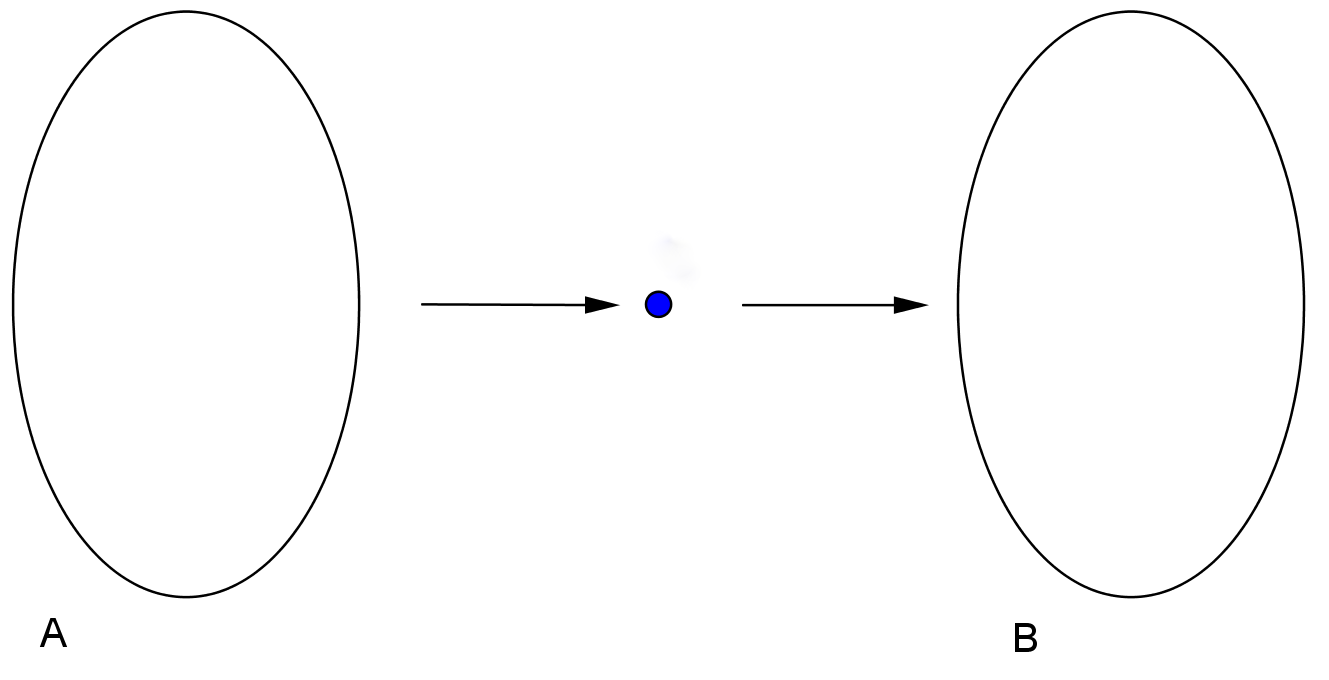
\includegraphics[scale=0.8]{Prob_1.png}
\end{center}
 We know $|B|\geq1$ because in order for $k$ to be a queen in $W$ as we've said it is, all elements in $A$ must be beaten by at least one element in $B$. By the proof in problem one, we know that if a vertex is beaten, it is beaten by a queen. Therefore there must be a queen in $B$, and therefore there cannot possibly be exactly two queens in a tournament.
\end{proof}

\begin{problem}{3}
Please prove that there is no 4-tournament in which every vertex is a queen.
\end{problem}
 
\begin{proof}
If symmetry is taken into account, then there are four distinct possibilities for edges in an unlabeled 4-tournament, each distinguishable by a singular trait.
\begin{enumerate}
\item[(a)] One vertex beats all other vertices
\item[(b)] One vertex is beaten by all other vertices
\item[(c)] A combination of a and b
\item[(d)] There is a cycle between all four vertices of the graph
\end{enumerate}
Case (a) always results in only one queen, since the vertex which beats all other vertices has an indegree of 0, and therefore no other vertex can possibly satisfy the queen conditions. Case (b) can never result in every vertex being a queen because the vertex which is beaten by all other vertices has an outdegree of $0$, and therefore cannot possibly be a queen. Case (c) cannot result in all vertices being a queen due to both reasons given against case (a) and case (b). This leaves case (d). After satisfying the case condition that there be a cycle between all four vertices, there remains two edges to be drawn, as in the example image below.
\begin{center}
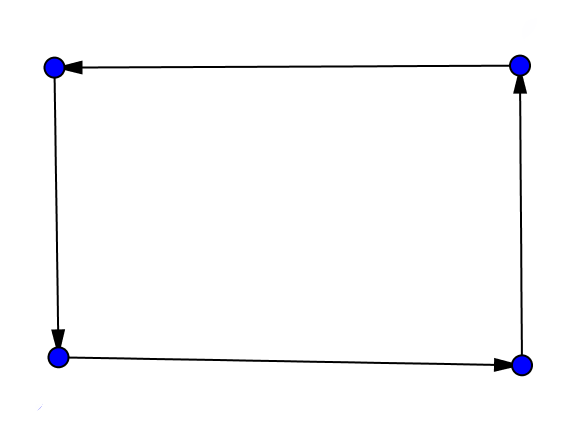
\includegraphics[scale=0.8]{Prob_3_1.png}
\end{center}
Regardless of how the two remaining edges are drawn, there will always be a vertex (we'll call it $p$ for peasant) with an indegree of $2$ that beats a vertex with an indegree of $2$, and so it is clear that $p$ cannot satisfy the queen condition, resulting in only $3$ queens in the tournament. This exhausts all possibilities for queens in a 4-tournament, and so it is impossible to have a 4-tournament in which every vertex is a queen.
\end{proof}

\end{document}